\chapter{Numerical Experiments}
\section{Constant Velocity Case - Subsonic}
\begin{figure}[H]
  \centering
  \begin{subfigure}{0.45\textwidth}
    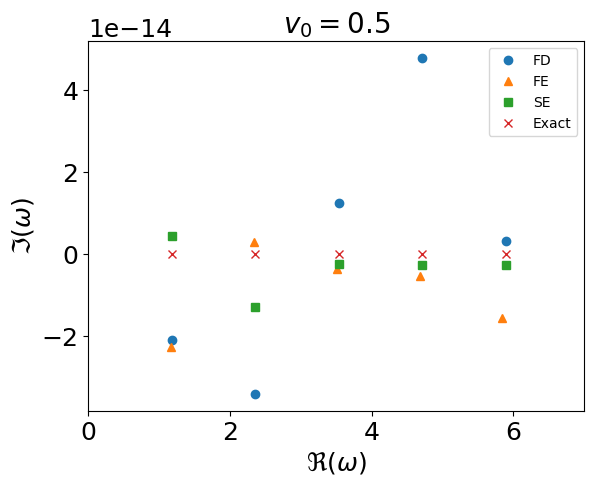
\includegraphics[width=0.9\linewidth]{figures/numerical-experiments/fixed-fixed/constant-v-v0=0.5}
    \caption{Dirichlet boundary, all modes are stable.}
  \end{subfigure}%
  \begin{subfigure}{0.45\textwidth}
    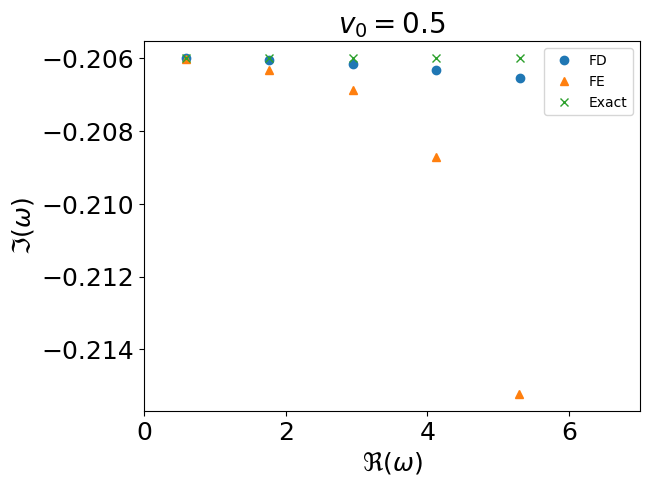
\includegraphics[width=\linewidth]{figures/numerical-experiments/fixed-open/constant-v-v0=0.5}
    \caption{Fixed-open boundary, all modes are stable.}
  \end{subfigure}
  \caption{Showing the first 5 eigenvalues. In the Dirichlet boundary case, all methods are close to the exact eigenvalues. Meanwhile, finite-difference method has higher accuracy than finite-element method in fixed-open case.}
  \label{fig:constant-v-subsonic}
\end{figure}

\section{Constant Velocity Case - Supersonic}
\begin{figure}[H]
  \begin{subfigure}{0.45\textwidth}
    \centering
    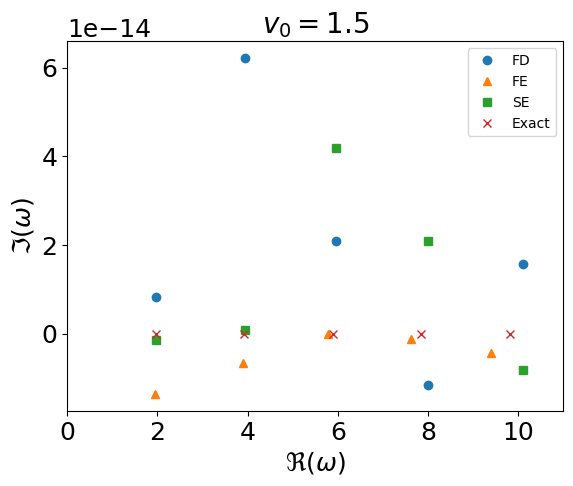
\includegraphics[width=0.9\linewidth]{figures/numerical-experiments/fixed-fixed/constant-v-v0=1.5}
    \caption{Dirichlet boundary, filtered modes are stable.}
  \end{subfigure}%
  \begin{subfigure}{0.45\textwidth}
    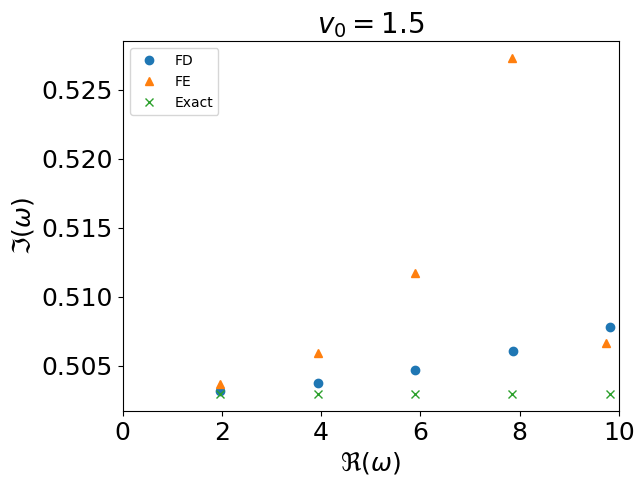
\includegraphics[width=\linewidth]{figures/numerical-experiments/fixed-open/constant-v-v0=1.5}
    \caption{Fixed-open boundary, all modes are unstable.}
  \end{subfigure}
  \caption{Showing the first 5 eigenvalues. In the Dirichlet boundary case, all methods are close to the exact eigenvalues. Meanwhile, finite-difference method has higher accuracy than finite-element method in fixed-open case.}
  \label{fig:constant-v-supersonic}
\end{figure}

\section{Error}
Because the existence of exact solution to problems Eq.(\ref{eq:polynomial-eigenvalue-problem}). The case with constant velocity profile is used as a sanity check. It allows us to verify the correctness of each method's implementation. This also serves as a reference to the accuracy spectral methods can achieve.

From Fig.\ref{fig:constant-v-subsonic} and Fig.\ref{fig:constant-v-supersonic}, we see that the order of growth rates is about $~10^{-14}$ for both subsonic and supersonic cases if the boundary condition is Dirichlet. We will use it a reference to the accuracy of our numerical methods. If a method produces growth rates with order close to $10^{-14}$, we consider the growth rates to be 0.

\begin{table} [H]
	\centering
	\caption{Relative error of each eigenvalue.}
	\begin{tabular}{|c|c|c|c|c|c|}
		\hline
		$v_0=0.5$   & 1 & 2 & 3 & 4 & 5 \\
		\hline
		FD & 2.827e-05 & 1.130e-04 & 2.541e-04 & 4.512e-04 & 7.040e-04 \\
		\hline
		FE & 0.005 & 0.005 & 0.006 & 0.008 & 0.010  \\
		\hline
		SE & 2.896e-05 & 1.157e-04 & 2.603e-04 & 4.626e-04 & 7.217e-04 \\
		\hline
	\end{tabular}
	\begin{tabular}{|c|c|c|c|c|c|}
		\hline
		$v_0=1.5$   & 1 & 2 & 3 & 4 & 5 \\
		\hline
		FD & 0.001 & 0.005 & 0.010 & 0.019 & 0.030 \\
		\hline
		FE & 0.006 & 0.010 & 0.019 & 0.029 & 0.043  \\
		\hline
		SE & 0.001 & 0.005 & 0.011 & 0.019 & 0.030 \\
		\hline
	\end{tabular}
	\label{table:eigenvalue-error-fixed-fixed}
\end{table}

\begin{table} [H]
	\centering
	\caption{Relative error of each eigenvalue. Notice that the ground mode for subsonic case is non-zero.}
	\begin{tabular}{|c|c|c|c|c|c|}
		\hline
		$v_0=0.5$   & 0 & 1 & 2 & 3 & 4 \\
		\hline
		FD & 1.209e-05 & 3.458e-05 & 5.775e-05 & 8.153e-05 & 1.061e-04 \\
		\hline
		FE & 8.090e-05 & 2.007e-04 & 2.981e-04 & 6.596e-04 & 1.821e-03  \\
		\hline
	\end{tabular}
	\begin{tabular}{|c|c|c|c|c|c|}
		\hline
		$v_0=1.5$   & 1 & 2 & 3 & 4 & 5 \\
		\hline
		FD & 9.163e-05 & 2.435e-04 & 4.833e-04 & 8.160e-04 & 1.243e-03 \\
		\hline
		FE & 4.431e-04 & 7.924e-04 & 1.516e-03 & 3.103e-03 & 8.001e-03  \\
		\hline
	\end{tabular}
	\label{table:eigenvalue-error-fixed-open}
\end{table}

\begin{figure}[H]
	\centering
	\begin{subfigure}{0.5\textwidth}
		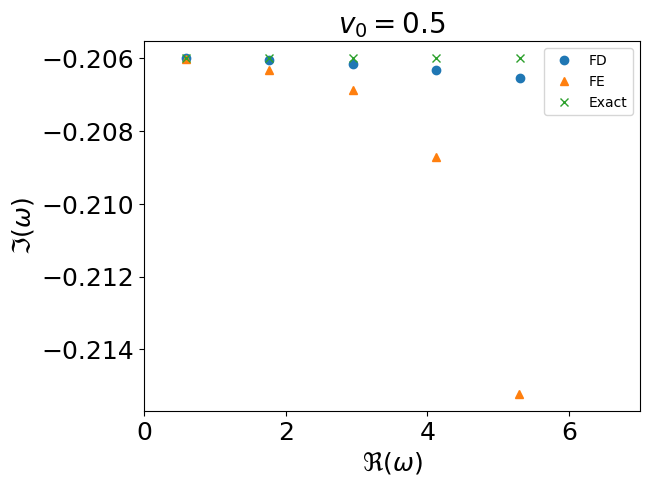
\includegraphics[width=\linewidth]{figures/numerical-experiments/fixed-open/constant-v-v0=0.5}
		\caption{All modes are stable.}
	\end{subfigure}%
	\begin{subfigure}{0.5\textwidth}
		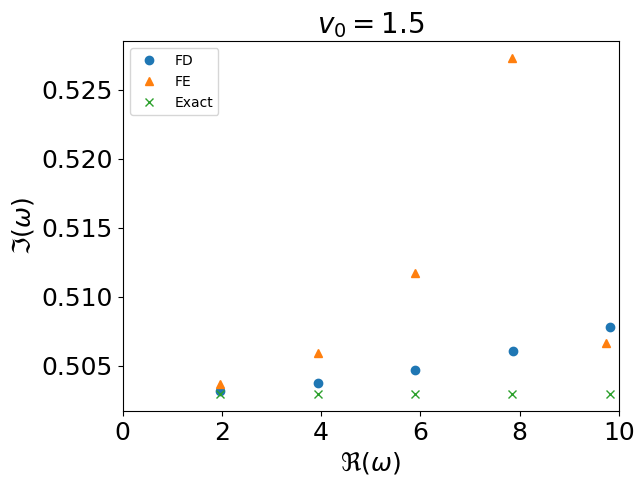
\includegraphics[width=\linewidth]{figures/numerical-experiments/fixed-open/constant-v-v0=1.5}
		\caption{All modes are unstable.}
	\end{subfigure}
	\caption{Showing the first 5 eigenvalues of each method. Finite-difference method has much better accuracy than finite-element method.}
	\label{fig:constant-v-fixed-open}
\end{figure}


\section{Subsonic Case}
\begin{figure} [H]
  \centering
  \begin{subfigure}{0.45\textwidth}
    \centering
    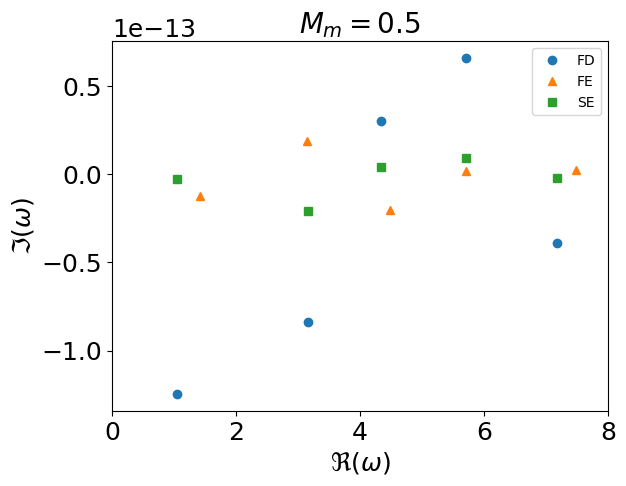
\includegraphics[width=\linewidth]{figures/numerical-experiments/fixed-fixed/subsonic-v}
    \caption{Dirichlet boundary, all modes are stable.}
  \end{subfigure}%
  \begin{subfigure}{0.45\textwidth}
    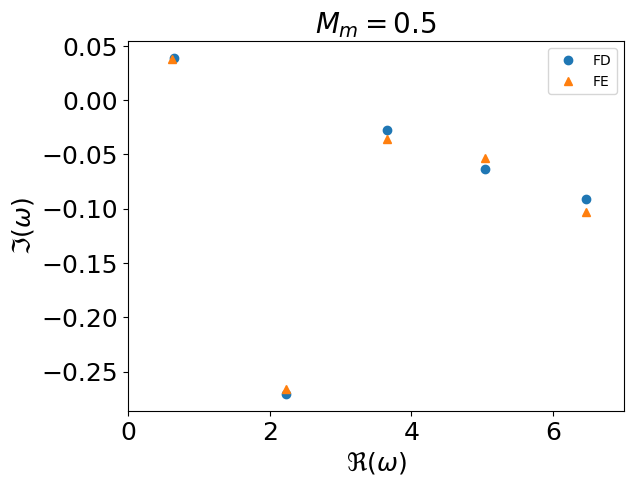
\includegraphics[width=\linewidth]{figures/numerical-experiments/fixed-open/subsonic-v}
    \caption{The ground mode is unstable, other modes are stable.}
  \end{subfigure}
  \caption{Showing the first 5 modes. It suggests that the subsonic flow in magnetic nozzle is stable.}
\end{figure}

\section{Supersonic Case}
\begin{figure} [H]
  \centering
  \begin{subfigure}{0.45\textwidth}
    \centering
    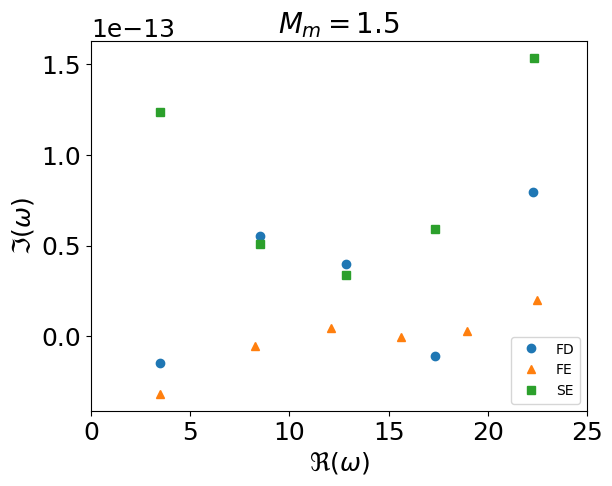
\includegraphics[width=\linewidth]{figures/numerical-experiments/fixed-fixed/supersonic-v}
    \caption{Dirichlet boundary, filtered modes are stable.}
  \end{subfigure}%
  \begin{subfigure}{0.45\textwidth}
    \centering
    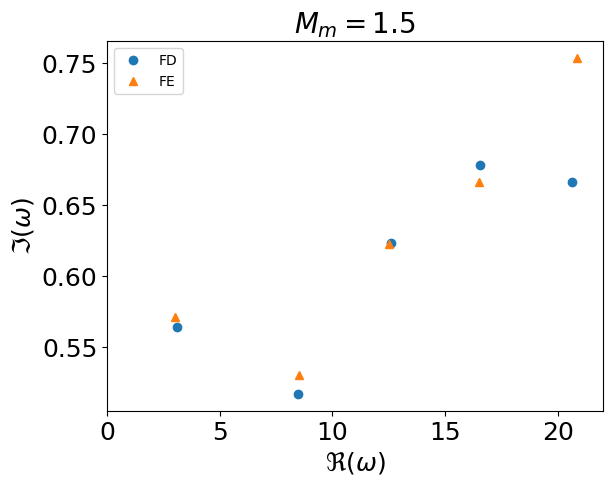
\includegraphics[width=\linewidth]{figures/numerical-experiments/fixed-open/supersonic-v}
    \caption{Fixed-open boundary, all modes are unstable.}
  \end{subfigure}
  \caption{This suggests that the supersonic flow is stable if the boundary is Dirichlet and unstable if the boundary is left-fixed-right-open.}
\end{figure}


\section{Accelerating Case}
Starting from the singular point, we shoot the solution to the left boundary. We find the set of eigenvalues such that $\tilde{v}(-1)=0$. With these eigenvalues, we can extend the solution to the supersonic region $(0,1]$. The first five eigenvalues are drawn in the graph.
\begin{figure} [H]
	\centering
	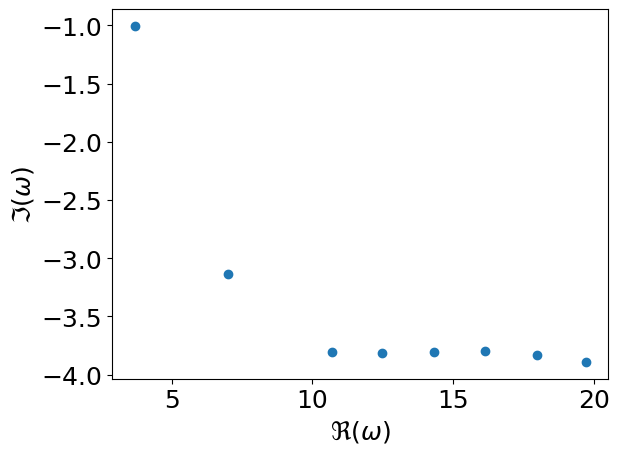
\includegraphics[width=0.7\linewidth]{figures/numerical-experiments/accelerating-v}
	\caption{All modes are stable.}
	\label{fig:accelerating-v}
\end{figure}
